\chap{ Implementing Algorithms in Hardware}
This is an exercise in using algorithmic state machine charts to implement algorithms as hardware circuits.
\section{Background}
Algorithmic State Machine (ASM) charts are a design tool that allow the specification of digital systems in a form similar to a flow chart. An example of an ASM chart is shown in Figure 11.1. It represents a circuit that counts the number of bits set to 1 in an n-bit input A $(A = a_{n-1}a_{n-2}. . .a_1a_0)$. The rectangular boxes in this diagram represent the states of the digital system, and actions specified inside of a state box occur on each active clock edge in this state. Transitions between states are specified by arrows. The diamonds in the ASM chart represent conditional tests, and the ovals represent actions taken only if the corresponding conditions are either true (on an arrow labeled 1) or false (on an arrow labeled 0).\\
\begin{figure}[h]
    \centering
    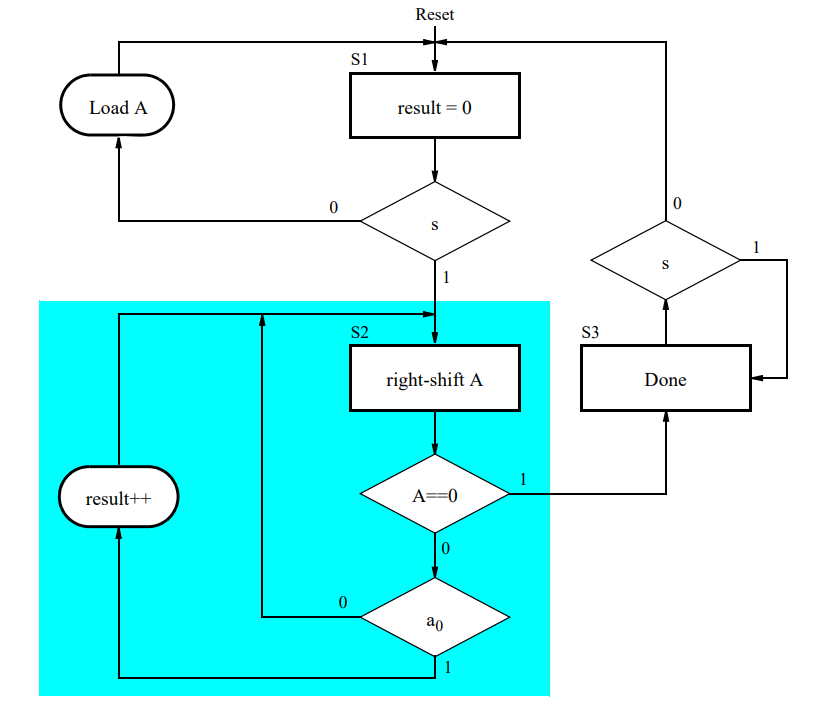
\includegraphics[scale = 0.65]{source/picture/Lab11/11.png}
    \caption{ASM chart for a bit counting circuit.}
\end{figure}
In this ASM chart, state S1 is the initial state. In this state the result is initialized to 0, and data is loaded into a register A, until a start signal, s, is asserted. The ASM chart then transitions to state S2, where it increments the result to count the number of 1’s in register A. Since state S2 specifies a shifting operation, then A should be implemented as a shift register. Also, since the result is incremented, then this variable should be implemented as a counter. When register A contains 0 the ASM chart transitions to state S3, where it sets an output Done = 1 and waits for the signal s to be deasserted.



%%%%%%%%%%%%%%%%%%%%%%%%%%%%%%%%%%%%%%%%%%%%%
\section{Part I}
\begin{itemize}
    \item []\textbf{REQUIREMENT}
        \begin{enumerate}
            \item Write Verilog code to implement the bit-counting circuit using the ASM chart shown in Figure 1 on a DE-series board. Include in your Verilog code the datapath components needed, and make an FSM for the control circuit.
            \item The inputs to your circuit should consist of an 8-bit input connected to slide switches $W_{7-0}$, a synchronous reset connected to $KEY_0$, and a start signal (s) connected to switch $SW_9$. Use the 50 MHz clock signal provided on the board as the clock input for your circuit. Be sure to synchronize the s signal to the clock.
            \item Display the number of 1s counted in the input data on the 7-segment display $HEX_0$, and signal that the algorithm is finished by lighting up $LEDR_9$.\\
        \end{enumerate}
    \item []\textbf{SOLUTION}
        \begin{itemize}
            \item []In this lab, we were introduced to the \textbf{datapath} definition. A finite State Machine is used to control what is plane to be done in its state, another component in the design is the \textbf{datapath}.
            \item []Based on the idea of the datapath of part 1, we constructed the datapath as follows. 
                \begin{lstlisting}[language=verilog]
//Datapath
always @(posedge flag) begin
        case (status)
            INIT: 	if (S==1'b1) 	status <= BEGIN;
            BEGIN: 	if (a==0) 		status <= END;
            END: 		if (S==1'b0)	status <= INIT;
            default: status <= INIT;
        endcase
end
                \end{lstlisting}
            \item []The FSM for this part
                \begin{lstlisting}[language=verilog]
//FSM Control
always @(posedge flag) begin
    case (status)
        INIT: begin
            count 	<= 0;
            DONE		<= 0;
            a 			<= DATA_IN;
        end
        BEGIN: begin
            if (a[0]==1'b1) count <= count + 1;
            a			<= a>>1;
        end
        END: begin
            DONE		<= 1;
        end
        default: status <= INIT;
    endcase
end
                \end{lstlisting}
        \end{itemize}
    \item []\textbf{VERIFICATION}
        \begin{itemize}
            \item [] As we can see, our DIN is 00000011, which contains four 2s, and the result is exactly 2 at $t=65ns$ (7'b0100100 is the signal representing 2).
        \end{itemize}
        \begin{figure}[h]
            \centering
            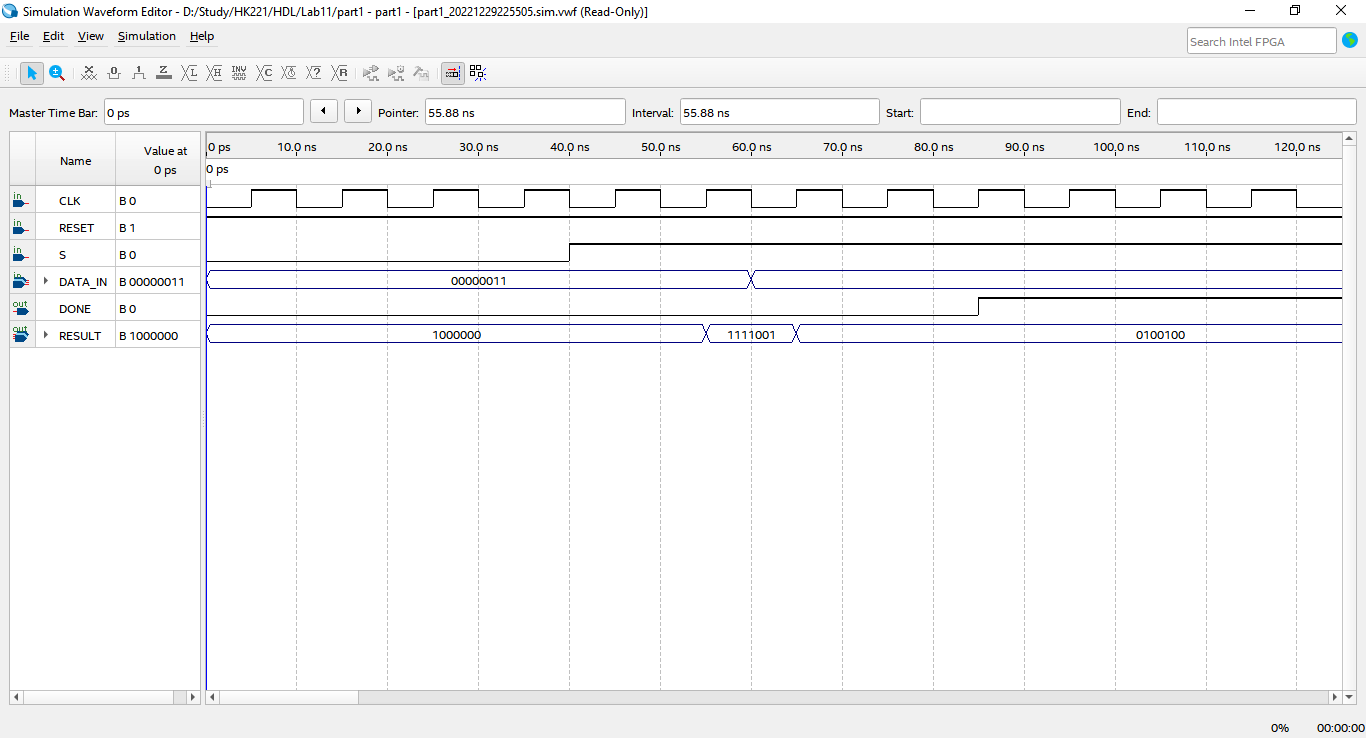
\includegraphics[width=\textwidth]{source/picture/Lab11/Lab11_1.png}
            \caption{Simulation result of the bit counter}
            \label{fig:my_label}
        \end{figure}
    
\end{itemize}

\newpage

\section{Part II}
\begin{itemize}
    \item []\textbf{REQUIREMENT} 
        \begin{enumerate}

            \item We wish to implement a binary search algorithm, which searches through an array to locate an 8-bit value $A$ specified via switches
                \begin{figure}[h]
                    \centering
                    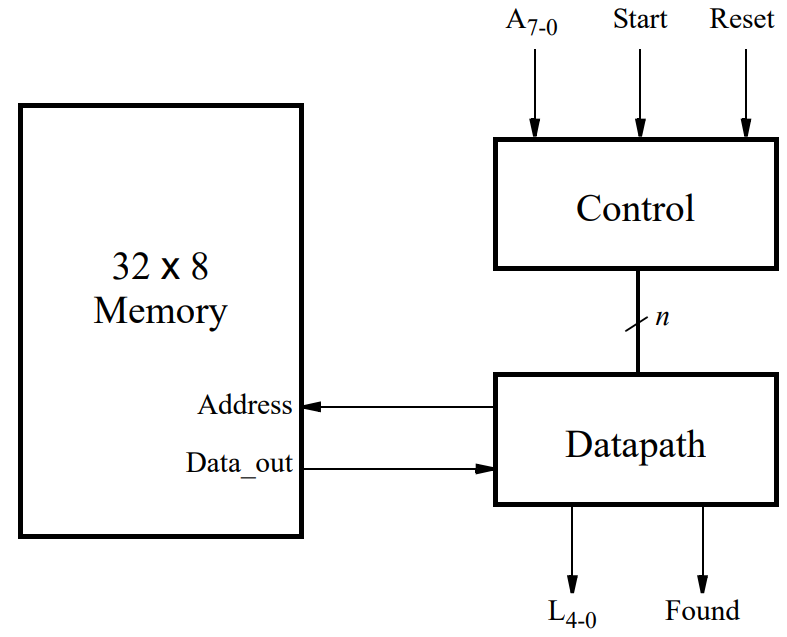
\includegraphics[width=4in]{source/picture/Lab11/Screenshot 2021-12-24 161403.png}
                    \caption{Block diagram for the binary search module}
                \end{figure}
            \item The binary search algorithm works on a sorted array. Rather than comparing each value in the array to the one being sought, we first look at the middle element and compare the sought value to the middle element. If the middle element has a greater value, then we know that the element we seek must be in the first half of the array. Otherwise, the value we seek must be in the other half of the array. By applying this approach recursively, we can locate the sought element in only a few steps. The algorithm for a binary search goes like this:
                \begin{lstlisting}[language=Python]
def binary_search(arr, low, high, x):
    if high >= low:
        mid = (high + low) // 2
        if arr[mid] == x:
            return mid
        elif arr[mid] > x:
            return binary_search(arr, low, mid - 1, x)
        else:
            return binary_search(arr, mid + 1, high, x)
    else:
        return -1
                \end{lstlisting} 
            \item In this circuit, the array is stored in a memory module that is implemented inside the FPGA chip. A diagram of the memory module that we need to create is depicted in Figure 11.5. This memory module has one read port and one write port, and is called a synchronous random-access memory (synchronous RAM). Note that the memory module includes registers for synchronously loading addresses, input data, and the Write input. These registers are required due to the design of the memory resources in the Intel FPGA chip.
                \begin{figure}[h]
                    \centering
                    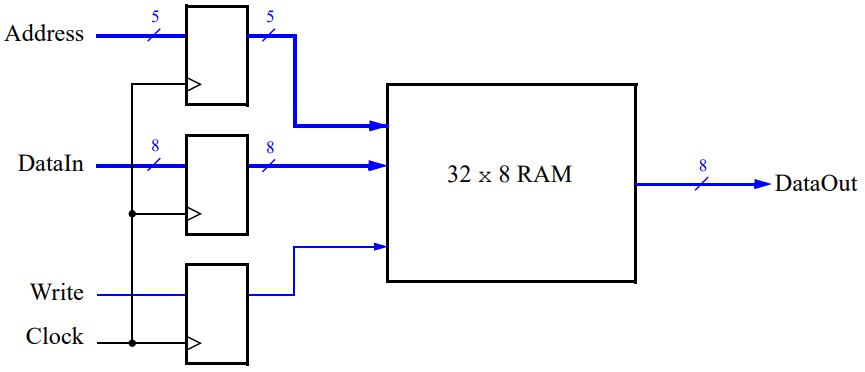
\includegraphics[width=5in]{source/picture/Lab11/image2.png}
                    \caption{The 32 $\times$ 8 RAM with address register}
                    \label{fig:my_label}
                \end{figure}
        \end{enumerate}
    \item []\textbf{SOLUTION} 
        \begin{itemize}
            \item []To place data into the memory, we need to specify initial values that should be stored in the memory once our circuit has been programmed into the FPGA chip. This can be done by initializing the memory using the contents of a memory initialization file (MIF). We have specified a file named my\_array.mif, which then has to be created in the folder that contains the Quartus project. The memory initialization file is given in below. We set the contents of our MIF file such that it contains a sorted collection of integers.
                \begin{lstlisting}[language=verilog]
WIDTH=8;
DEPTH=32;

ADDRESS_RADIX=HEX;
DATA_RADIX=HEX;

CONTENT BEGIN
	00  :   01;
	01  :   02;
	02  :   03;
	03  :   05;
	[04..05]  :   06;
	06  :   07;
	[07..08]  :   08;
	09  :   0A;
	[0A..0B]  :   0B;
	0C  :   10;
	0D  :   11;
	[0E..0F]  :   12;
	10  :   13;
	11  :   14;
	12  :   15;
	13  :   17;
	14  :   18;
	[15..16]  :   19;
	17  :   1A;
	18  :   1B;
	19  :   1C;
	1A  :   1D;
	[1B..1C]  :   1E;
	[1D..1E]  :   1F;
	1F  :   20;
END;
                \end{lstlisting}
            \item []After creating the MIF file, we started to code the actual Binary Search module. But first, as with part 1, we need an ASM chart for such module.
                \begin{figure}[h]
                    \centering
                    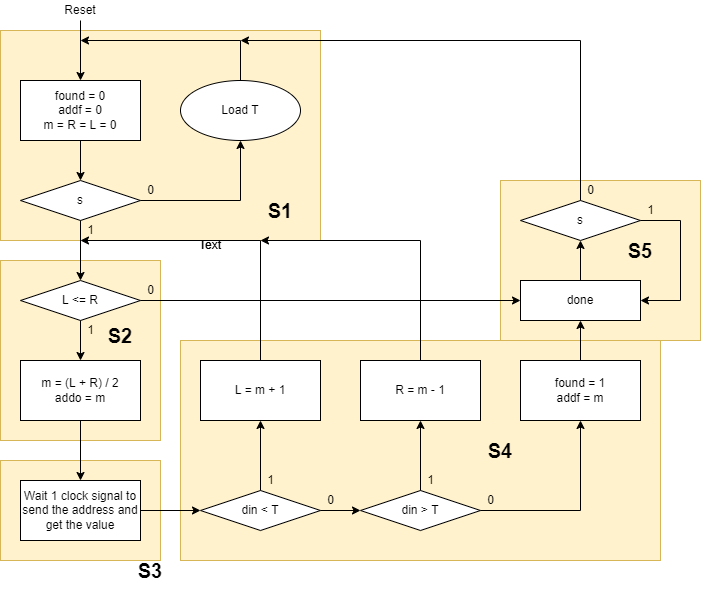
\includegraphics[width=6in]{source/picture/Lab11/asm.drawio.png}
                    \caption{ASM chart for a binary search circuit}
                    \label{fig:my_label}
                \end{figure} 
            \item [] Based on the idea of the datapath of part 1, we constructed the datapath as follows.
                \begin{lstlisting}[language=verilog]
//Datapath
always @(posedge flag) begin
    case (status)
        INIT:		if (START==1)		status <= BEGIN;
        BEGIN: begin	
                    if (done==1) 		status <= END;
                    else					status <= WAIT;
                 end
        WAIT:								status <= FIND;
        FIND:								status <= BEGIN;
        END:		if (START==0)		status <= INIT;
    endcase
end
                \end{lstlisting}
            \item []About the FSM, we have 5 states. In the beginning, we just design with 4 states:
                \begin{itemize}
                    \item \textbf{INIT}: initialize some value and load DATA\_IN into a reg.
                    \item \textbf{BEGIN}: calculate the address of the value needed to compare with the DATA\_IN.
                    \item \textbf{FIND}:  execute the comparison
                    \item \textbf{DONE}: our system change to this state if found the address of DATA\_IN inside the memory, or even if it couldn’t be found after looked the whole memory.
                \end{itemize}
            \item []After try this state machine, we noticed that because every work is executed only in that state, so after changing the state, it has to wait for another clock to execute the job of the new state. So if we use the FSM above, the memory couldn’t have  enough time to load the value of the address we need.
            \item []We decided to add another state, named WAIT, to wait for the memory to load the value of the memory.
                \begin{lstlisting}[language=verilog]
//FSM Control
always @(posedge flag) begin
    case (status)
        INIT: begin
            data_temp 	<= DATA_IN;
            left			<= 5'b00000;
            right			<= 5'b11111;
            address_out <= 5'b00000;
            
            done			<= 0;
            FOUND			<= 0;
        end
        BEGIN: begin
            address_out <= (left+right)/2;
        end
        FIND: begin
            if (data_temp > value_out) 		left 	<= address_out+1;
            else if (data_temp < value_out)  right <= address_out-1;
            else if (data_temp == value_out)begin 
                done	<= 1;
                FOUND <= 1;
            end
            else if (left >= right) begin
                done 	<= 1;
                FOUND <= 0;
            end
        end
    
    endcase
end
                \end{lstlisting}
        \end{itemize}
\end{itemize}
\newpage